\section{实验结果与分析}

\subsection{QMIX 主实验结果}

\begin{table}[H]
  \centering
  \caption{QMIX 主实验结果}
  \label{tab:qmix-main-results}
  \resizebox{\linewidth}{!}{
  \begin{tabular}{llrrrrr}
    \toprule
    地图 & 变体 & Seeds & Final Win & Best Win & Win AUC & Wall Hours \\
    \midrule
    \code{5m\_vs\_6m} & \code{qmix} & 3/3 & 0.6250 & 0.7813 & 0.3926 & 6.59 \\
    \code{5m\_vs\_6m} & \code{qmix\_attnres} & 3/3 & 0.5417 & 0.7188 & 0.4111 & 15.14 \\
    \code{5m\_vs\_6m} & \code{qmix\_attnres\_l2} & 3/3 & 0.6042 & 0.8021 & 0.4493 & 8.29 \\
    \code{5m\_vs\_6m} & \code{qmix\_attnres\_block} & 3/3 & 0.5000 & 0.6875 & 0.3951 & 13.97 \\
    \code{5m\_vs\_6m} & \code{qmix\_depth\_mlp} & 3/3 & 0.4583 & 0.7396 & 0.4114 & 8.40 \\
    \midrule
    \code{3s5z} & \code{qmix} & 3/3 & 0.9167 & 1.0000 & 0.7717 & 9.15 \\
    \code{3s5z} & \code{qmix\_attnres} & 3/3 & 0.9375 & 1.0000 & 0.7504 & 18.29 \\
    \code{3s5z} & \code{qmix\_attnres\_l2} & 3/3 & 0.9583 & 1.0000 & 0.7608 & 10.31 \\
    \code{3s5z} & \code{qmix\_attnres\_block} & 3/3 & 0.8750 & 1.0000 & 0.7493 & 16.61 \\
    \code{3s5z} & \code{qmix\_depth\_mlp} & 3/3 & 0.9896 & 1.0000 & 0.7417 & 10.84 \\
    \bottomrule
  \end{tabular}}
\end{table}


从 \code{5m\_vs\_6m} 结果看，原始 QMIX 的 final win rate 为 0.6250。
重型 \code{qmix\_attnres} 和 \code{qmix\_attnres\_block} 的 final win rate 分别为 0.5417 和 0.5000，未能稳定超过 baseline。
\code{qmix\_attnres\_l2} 的 best win rate 和 win-rate AUC 分别达到 0.8021 和 0.4493，高于 QMIX 的 0.7813 和 0.3926，但 final win rate 为 0.6042，仍略低于 QMIX。

从 \code{3s5z} 结果看，多数方法 best win rate 均达到 1.0000，说明该地图在当前设置下区分度较弱。
因此，\code{3s5z} 更适合作为 sanity check，而不宜作为强结论地图。

\begin{table}[H]
  \centering
  \caption{\code{5m\_vs\_6m} 上 QMIX 变体的结构复杂度与训练成本摘要。Wall Ratio 以 QMIX baseline 的平均训练时间为 1.00。}
  \label{tab:model-cost-summary}
  \resizebox{\linewidth}{!}{
  \begin{tabular}{llrrrrl}
    \toprule
    变体 & Attention Mode & Layers & Wall Ratio & Final Win & Win AUC & 结论 \\
    \midrule
    \code{qmix} & - & 0 & 1.00 & 0.6250 & 0.3926 & baseline \\
    \code{qmix\_attnres} & full & 4 & 2.30 & 0.5417 & 0.4111 & 成本高，final win 下降 \\
    \code{qmix\_attnres\_l2} & full & 2 & 1.26 & 0.6042 & 0.4493 & AUC 较高，final win 不稳定 \\
    \code{qmix\_attnres\_block} & block & 4 & 2.12 & 0.5000 & 0.3951 & 成本高，收益不明显 \\
    \code{qmix\_depth\_mlp} & none & 4 & 1.28 & 0.4583 & 0.4114 & 单纯加深不能解释收益 \\
    \bottomrule
  \end{tabular}}
\end{table}


表~\ref{tab:model-cost-summary} 进一步比较了结构复杂度、训练成本和主要性能指标。
在 \code{5m\_vs\_6m} 上，Full 与 Block 版本的平均训练时间分别约为 QMIX 的 2.30 倍和 2.12 倍，但 final win 均低于 baseline。
AttnRes-L2 的 wall-time ratio 降至 1.26，且 AUC 高于 QMIX，但 final win 仍未稳定超过 baseline。
Depth-only control 的 final win 明显下降，说明当前结果不能简单解释为“增加后处理网络深度即可带来收益”。

\begin{figure}[H]
  \centering
  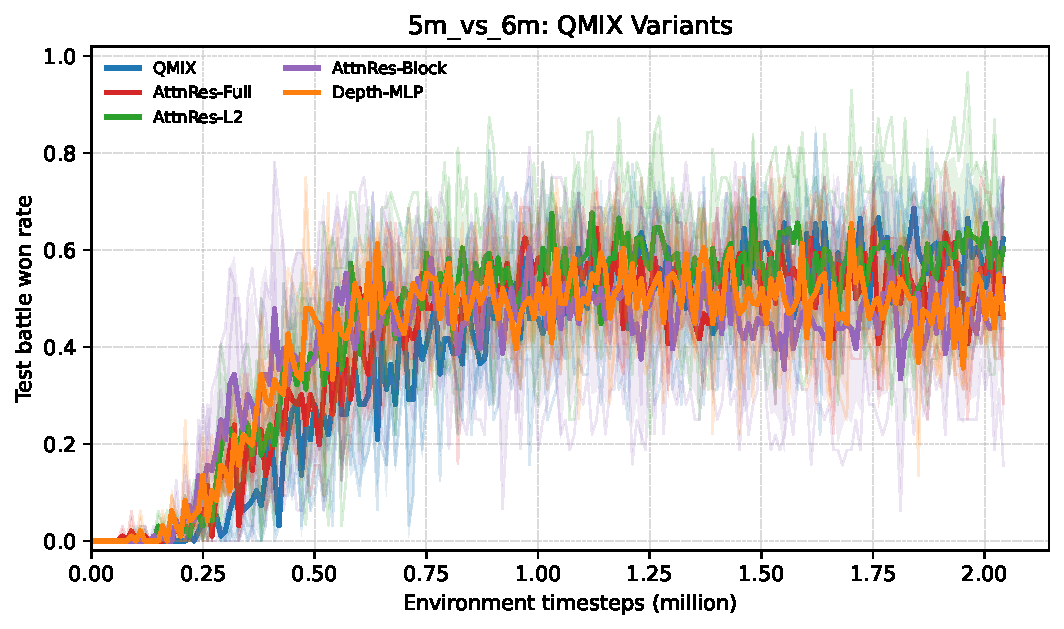
\includegraphics[width=0.92\linewidth]{figures/5m_vs_6m_qmix_win_curve.pdf}
  \caption{\code{5m\_vs\_6m} 上 QMIX 主实验变体的测试胜率学习曲线。曲线为 3 个 seeds 的均值，阴影表示标准差，浅色细线表示单个 seed。}
  \label{fig:5m-qmix-win-curve}
\end{figure}

\begin{figure}[H]
  \centering
  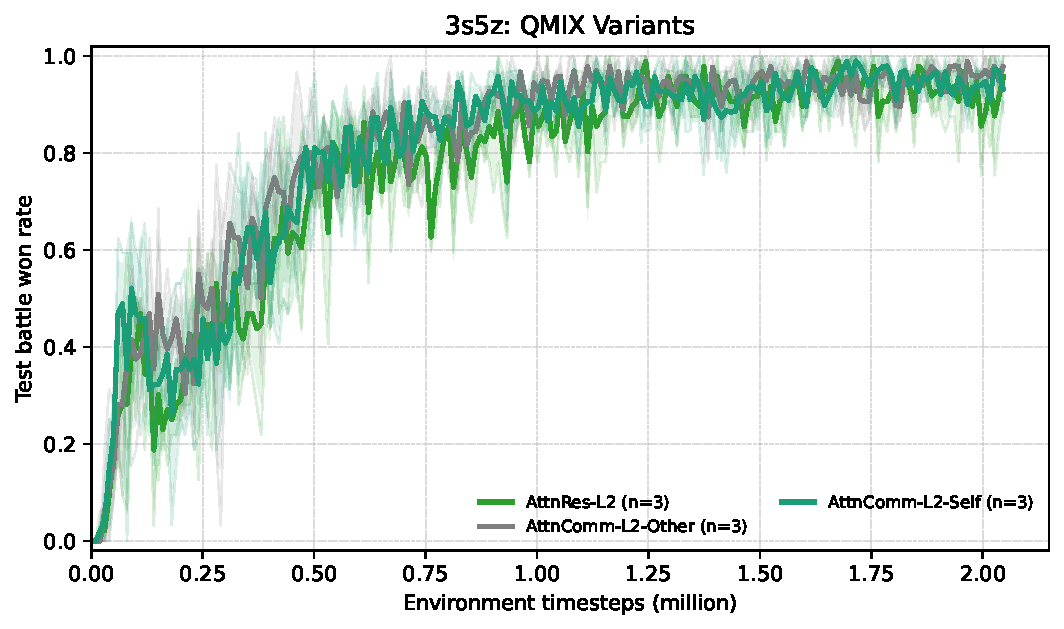
\includegraphics[width=0.92\linewidth]{figures/3s5z_qmix_win_curve.pdf}
  \caption{\code{3s5z} 上 QMIX 主实验变体的测试胜率学习曲线。曲线为 3 个 seeds 的均值，阴影表示标准差，浅色细线表示单个 seed。}
  \label{fig:3s5z-qmix-win-curve}
\end{figure}

\subsection{Depth-only Control 分析}

\code{qmix\_depth\_mlp} 在 \code{5m\_vs\_6m} 上的 final win rate 为 0.4583，低于 QMIX。
这说明单纯增加后处理网络深度并不能稳定带来收益。
该对照支持本文的分析重点：当前问题不是“网络加深一定有效”，而是需要判断选择性聚合机制是否真正适配 MARL agent。

\subsection{跨算法轻量 AttnRes-L2 验证}

\begin{table}[H]
  \centering
  \caption{跨算法轻量 AttnRes-L2 对照结果}
  \label{tab:cross-algorithm-results}
  \resizebox{\linewidth}{!}{
  \begin{tabular}{lllrrrrl}
    \toprule
    地图 & Baseline & Candidate & Paired Seeds & $\Delta$ Final Win & $\Delta$ Best Win & $\Delta$ AUC & 解释 \\
    \midrule
    \code{5m\_vs\_6m} & \code{iql} & \code{iql\_attnres\_l2} & 3 & +0.0833 & +0.1458 & +0.0455 & lightweight transfer 有正向信号 \\
    \code{5m\_vs\_6m} & \code{vdn} & \code{vdn\_attnres\_l2} & 3 & +0.0625 & +0.0104 & +0.0577 & AUC 提升但 seed 表现混合 \\
    \code{5m\_vs\_6m} & \code{qmix} & \code{qmix\_attnres\_l2} & 3 & -0.0208 & +0.0208 & +0.0567 & mixed or unstable \\
    \bottomrule
  \end{tabular}}
\end{table}


跨算法结果显示，AttnRes-L2 在 IQL、VDN 和 QMIX 三类 baseline 上均提高了平均 win-rate AUC，分别提升 0.0455、0.0577 和 0.0567。
这说明轻量化选择性聚合在学习过程中具有一定正向信号。
但是，final win rate 的表现并不一致：IQL 和 VDN 的平均 final win 分别提升 0.0833 和 0.0625，而 QMIX 的平均 final win 下降 0.0208。
从 paired seeds 看，VDN 的 final win 只在 1/3 seeds 上优于 baseline，AUC 在 2/3 seeds 上优于 baseline，因此更适合解释为 mixed or unstable，而不是稳定改进。
因此，本文仅将 AttnRes-L2 表述为具有 limited positive signal 的轻量化变体，不将其作为稳定优于既有价值分解方法的新算法。

\begin{table}[H]
  \centering
  \caption{\code{5m\_vs\_6m} 上 AttnRes-L2 的 paired seed delta。Delta 为 candidate 减 baseline。}
  \label{tab:paired-seed-delta}
  \resizebox{\linewidth}{!}{
  \begin{tabular}{llrrrrl}
    \toprule
    Baseline & Seed & Baseline Final & L2 Final & $\Delta$ Final & $\Delta$ AUC & Seed-level 判断 \\
    \midrule
    \code{iql} & 1 & 0.3750 & 0.3125 & -0.0625 & +0.0412 & mixed \\
    \code{iql} & 2 & 0.3750 & 0.6563 & +0.2813 & +0.0580 & candidate better \\
    \code{iql} & 3 & 0.4063 & 0.4375 & +0.0313 & +0.0372 & candidate better \\
    \midrule
    \code{vdn} & 1 & 0.6563 & 0.6250 & -0.0313 & -0.0585 & candidate worse \\
    \code{vdn} & 2 & 0.5625 & 0.7813 & +0.2188 & +0.1138 & candidate better \\
    \code{vdn} & 3 & 0.6563 & 0.6563 & +0.0000 & +0.1177 & mixed \\
    \midrule
    \code{qmix} & 1 & 0.7500 & 0.6875 & -0.0625 & +0.0887 & mixed \\
    \code{qmix} & 2 & 0.4375 & 0.6563 & +0.2188 & +0.1528 & candidate better \\
    \code{qmix} & 3 & 0.6875 & 0.4688 & -0.2188 & -0.0714 & candidate worse \\
    \bottomrule
  \end{tabular}}
\end{table}


表~\ref{tab:paired-seed-delta} 给出了 seed-level paired delta。
可以看到，IQL 的 3 个 seeds 均获得正向 AUC delta，但 final win 仍有一个 seed 下降；VDN 和 QMIX 则同时出现 candidate better、mixed 和 candidate worse。
这说明 AttnRes-L2 在学习过程中确实存在一定 AUC 信号，但最终胜率对 seed 和后端价值分解方法较敏感。

\begin{figure}[H]
  \centering
  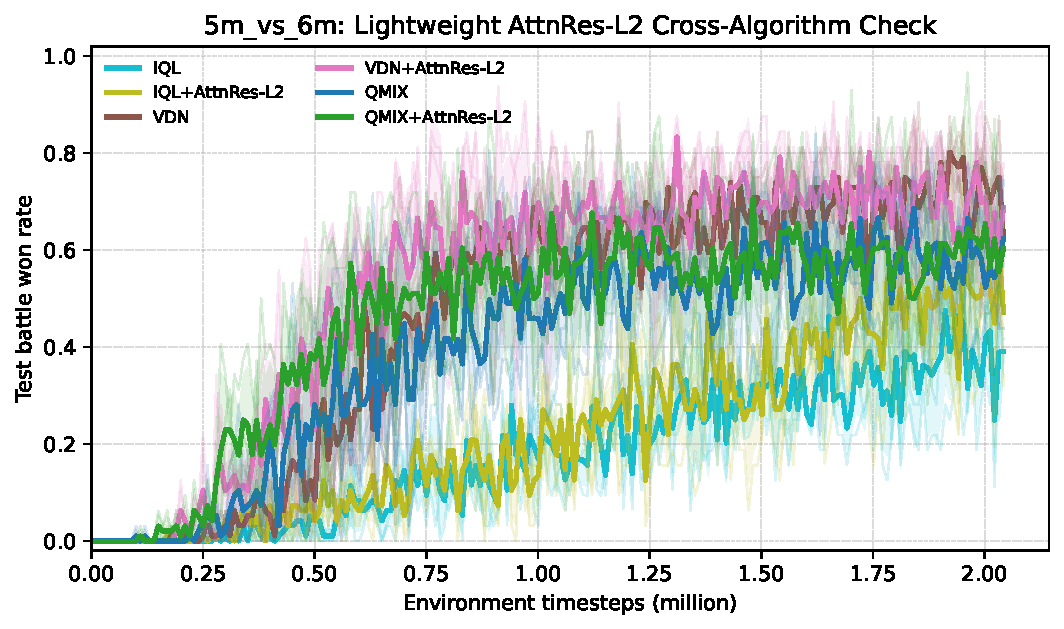
\includegraphics[width=0.92\linewidth]{figures/5m_vs_6m_cross_algorithm_win_curve.pdf}
  \caption{\code{5m\_vs\_6m} 上轻量 AttnRes-L2 的跨算法测试胜率曲线。曲线为 3 个 seeds 的均值，阴影表示标准差；图中包含 IQL、VDN、QMIX 及其 AttnRes-L2 变体。}
  \label{fig:cross-algorithm-win-curve}
\end{figure}

\subsection{Agent-wise Communication Extension}

前述结果表明，直接将 depth-wise Attention Residuals 插入浅层 recurrent agent 后并不能稳定形成 final win-rate 收益。
基于这一观察，本文进一步进行了一个小规模扩展实验：保持 QMIX learner、mixer 和动作选择器不变，只在 GRU hidden state 与 individual Q head 之间加入两层 agent-wise attention communication。
该扩展并不是替换 QMIX 算法，而是将 selective attention 从 depth dimension 转移到 agent dimension，用于检验跨智能体通信是否更符合 SMAC 的协同瓶颈。

\begin{table}[H]
  \centering
  \caption{\code{5m\_vs\_6m} 上 AttnComm-QMIX-L2 初步扩展结果（\(t_{\max}=5.0\)M）}
  \label{tab:attncomm-5m-extension}
  \resizebox{\linewidth}{!}{
  \begin{tabular}{lrrrrrr}
    \toprule
    变体 & Seeds & Final Win & Best Win & Win AUC & Wall Hours & 相对 QMIX AUC \(\Delta\) \\
    \midrule
    \code{qmix} & 3/3 & 0.5208 & 0.8021 & 0.4986 & 24.80 & -- \\
    \code{qmix\_attnres\_l2} & 3/3 & 0.5833 & 0.8021 & 0.5028 & 33.00 & +0.0043 \\
    \code{qmix\_attncomm\_l2\_other} & 3/3 & 0.6354 & 0.8542 & 0.5429 & 33.40 & +0.0444 \\
    \code{qmix\_attncomm\_l2\_self} & 3/3 & 0.5938 & 0.8646 & 0.5207 & 33.34 & +0.0222 \\
    \bottomrule
  \end{tabular}}
\end{table}


表~\ref{tab:attncomm-5m-extension} 给出了 \code{5m\_vs\_6m} 上 \(t_{\max}=5.0\)M 的完整 3-seed 初步结果。
在 3 个 paired seeds 上，\code{qmix\_attncomm\_l2\_other} 的 final win、best win 和 AUC 均高于 QMIX baseline，平均 final win 从 0.5208 提升到 0.6354，AUC 从 0.4986 提升到 0.5429，对应 final win \(+0.1146\)、AUC \(+0.0444\)。
\code{qmix\_attncomm\_l2\_self} 也取得正向均值提升，final win 和 AUC 分别提升 \(+0.0729\) 与 \(+0.0222\)，但幅度小于 other-only 版本。
从 paired comparison 看，other-only 版本在 final win 和 AUC 上均有 2/3 seeds 优于 baseline，self-inclusive 版本同样为 2/3 seeds 优于 baseline。
这说明 agent-wise communication attention 在当前设置下具有比 depth-wise hidden 后处理更直接的正向信号；同时，other-only 优于 self-inclusive 的现象也支持收益主要来自跨智能体信息聚合，而不只是额外的 self-attention 表示变换。

不过，该结果仍应谨慎解读。
首先，\code{qmix\_attnres\_l2} 在完整 3 seeds 后 final win 也高于 QMIX，但 AUC 增益仅为 \(+0.0043\)，best win 与 QMIX 持平，且 final win 标准差较大。
因此，完整 5M 对照并不支持“direct depth-wise transfer 已经稳定有效”的强结论，更适合表述为弱正向但高方差的结果。
其次，AttnComm 的平均 wall-clock time 约为 QMIX 的 1.35 倍，说明通信模块带来了额外成本，但该成本低于前文 heavy Full/Block AttnRes 的训练开销。
最后，当前 \code{3s5z} 的 AttnComm 运行仍不作为本文主结论依据，因此本文只将 \code{5m\_vs\_6m} 视为主要正向诊断结果，不声称跨地图稳定提升。

\begin{figure}[H]
  \centering
  \begin{subfigure}{0.48\linewidth}
    \centering
    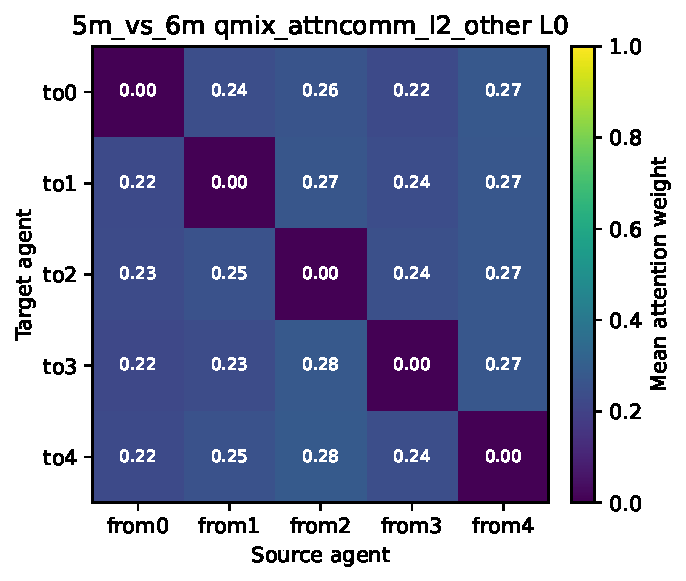
\includegraphics[width=\linewidth]{figures/5m_vs_6m_qmix_attncomm_l2_other_l0_attncomm_attention_heatmap.pdf}
    \caption{\code{other-only}, layer 0}
  \end{subfigure}
  \hfill
  \begin{subfigure}{0.48\linewidth}
    \centering
    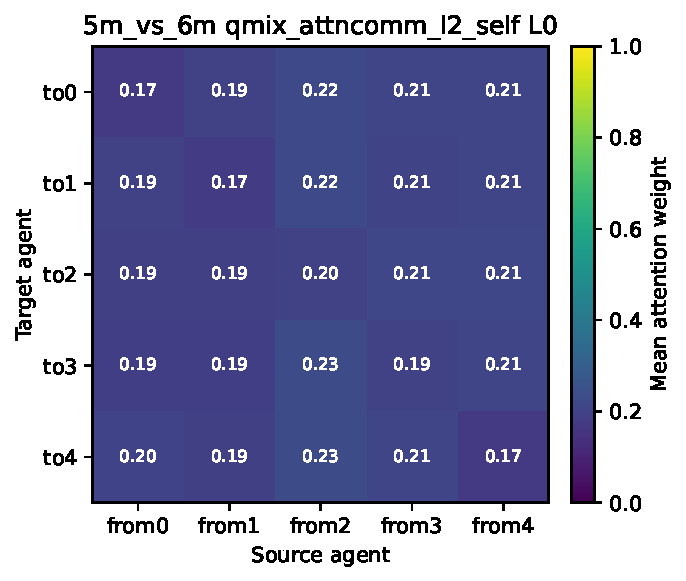
\includegraphics[width=\linewidth]{figures/5m_vs_6m_qmix_attncomm_l2_self_l0_attncomm_attention_heatmap.pdf}
    \caption{\code{self-inclusive}, layer 0}
  \end{subfigure}
  \caption{\code{5m\_vs\_6m} 上 AttnComm-L2 的 agent-to-agent attention heatmap。颜色表示跨 seeds 与日志点聚合后的平均 attention weight。}
  \label{fig:attncomm-heatmap}
\end{figure}

\subsection{训练效率分析}

训练时间显示，heavy variants 的成本显著高于 baseline。
在 \code{5m\_vs\_6m} 上，QMIX 平均训练时间约为 6.59 小时，而 \code{qmix\_attnres} 和 \code{qmix\_attnres\_block} 分别约为 15.14 小时和 13.97 小时。
\code{qmix\_attnres\_l2} 的成本约为 8.29 小时，明显低于重型版本，但仍高于 baseline。
在跨算法验证中，VDN+AttnRes-L2 的平均训练时间约为 VDN baseline 的 1.43 倍，进一步说明轻量化版本虽然比重型 AttnRes 更可控，但仍带来额外训练成本。
在 AttnComm 扩展实验中，两个通信变体的 wall-time ratio 约为 QMIX 的 1.35 倍。
这说明 agent-wise communication 相比原始 QMIX 仍有计算成本，但在当前 5M 训练设置下，其成本与收益之间呈现出比 heavy depth-wise AttnRes 更合理的折中。

\begin{figure}[H]
  \centering
  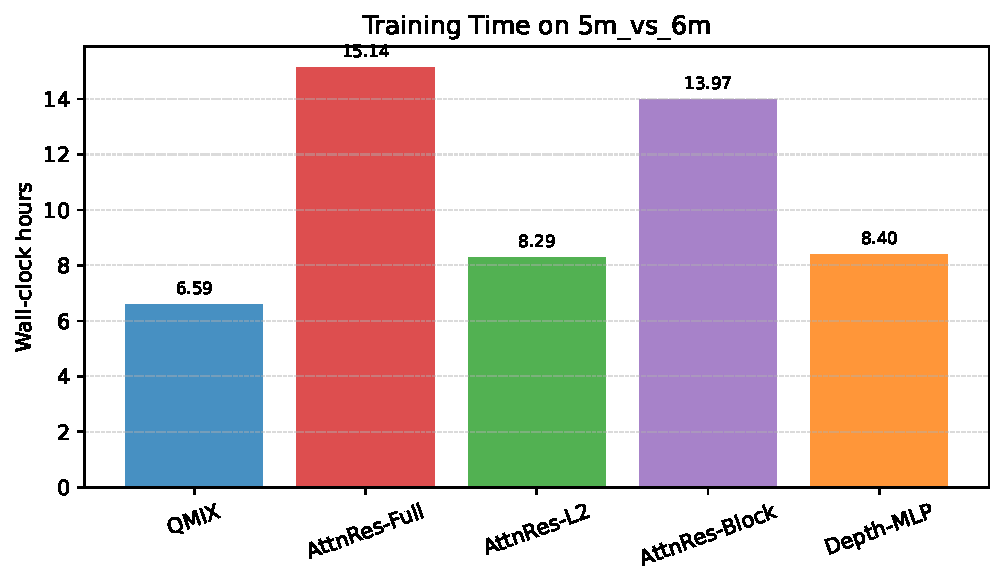
\includegraphics[width=0.82\linewidth]{figures/5m_vs_6m_wall_time_bar.pdf}
  \caption{\code{5m\_vs\_6m} 上各 QMIX 变体的平均训练墙钟时间。}
  \label{fig:wall-time-bar}
\end{figure}
